\documentclass[french,a4paper,18pt]{article}
\usepackage{graphicx} % Required for inserting images
\usepackage[style=authoryear, backend=biber]{biblatex}
\usepackage[left=1cm,right=1cm,top=1cm,bottom=2cm]{geometry}
\usepackage{hyperref}
\usepackage{csquotes}
\usepackage{animate}
\usepackage[T1]{fontenc}
\usepackage{amsmath}
\usepackage{multicol} % Package for multi-column layout
\usepackage[french]{babel}

\usepackage{listings}

\title{Apprentissage non-supervisé}
\author{Augustin Bresset | Guillaume Macquart De Terline}
\date{Février 2024}

\begin{document}

\maketitle

\begin{figure}[h]
    \centering
    
\includegraphics[scale=0.2]{images/logo-tsp-fond-blanc.png}
\end{figure}

\pagebreak

\twocolumn
% Your content here

\section{Introduction}

L'apprentissage non-supervisé est une branche de l'apprentissage automatique qui consiste à apprendre à partir de données non étiquetées. 
L'objectif est de trouver des structures dans les données, comme des groupes ou des clusters. 
L'apprentissage non-supervisé est souvent utilisé pour explorer des données et pour trouver des modèles cachés. 
Il est également utilisé pour la réduction de dimensionnalité, la visualisation de données et la génération de données.
Dans cet article nous allons étudier et comparer les algorithmes suivants : K-means, K-medoids DBSCAN et Modèle à Mélange de Gaussiennes.

Pour faire ceci, nous allons utiliser le jeu de données MNIST qui est un jeu de données de chiffres manuscrits.
Cela va nous permettre de facilement visualiser les résultats des algorithmes à travers un exemple concret.
On s'attend à ce que les algorithmes trouvent des clusters correspondant à des chiffres similaires. 
Cependant, il est important de noter que les algorithmes ne connaissent pas les étiquettes des chiffres et ne savent pas quels chiffres sont similaires.
C'est pourquoi on s'attend aussi à une confusion entre les chiffres similaires, comme le 3 et le 8 par exemple.

Enfin on va pouvoir comparer les performances des algorithmes en utilisant des métriques comme l'indice de silhouette.

\subsection{Base de données MNIST}
La base de données MNIST est un jeu de données de chiffres manuscrits. 
Chaque chiffre manuscrit est représenté par une image de 28x28 pixels 
Chaque pixel est représenté par un nombre entier entre 0 et 255, qui correspond à la luminosité du pixel.
Il y a 60 000 images dans l'ensemble d'entraînement et 10 000 images dans l'ensemble de test.

\begin{figure}[h!]
    \centering
    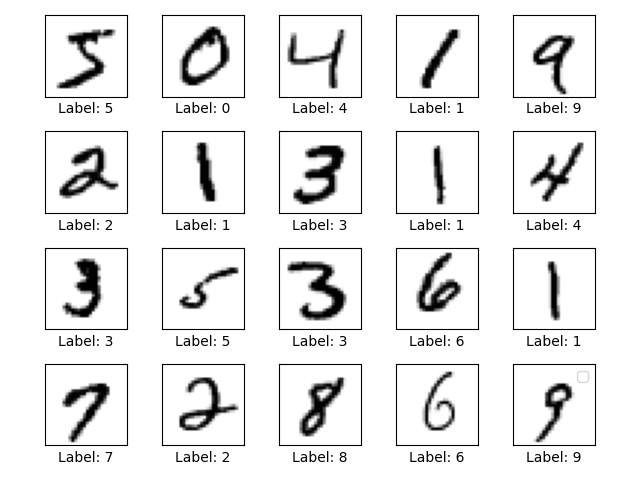
\includegraphics[scale=0.5]{images/mnist_plot.png}
    \caption{Exemple de chiffres de la base de données MNIST}\label{fig:mnist}
\end{figure}

Ce jeu de données est souvent utilisé pour tester des algorithmes de classification et de clustering.
On peut déjà remarqué ici la grande diversité des écritures des chiffres, ce qui rendra la tâche de clustering difficile.

\subsection{Présentation des modèles}
Pour montrer leur fonctionnement, on génère un jeu de données synthétique avec 300 points regroupés dans 5 clusters avec une variance de 0.8.
\begin{figure}[h]
    \centering
    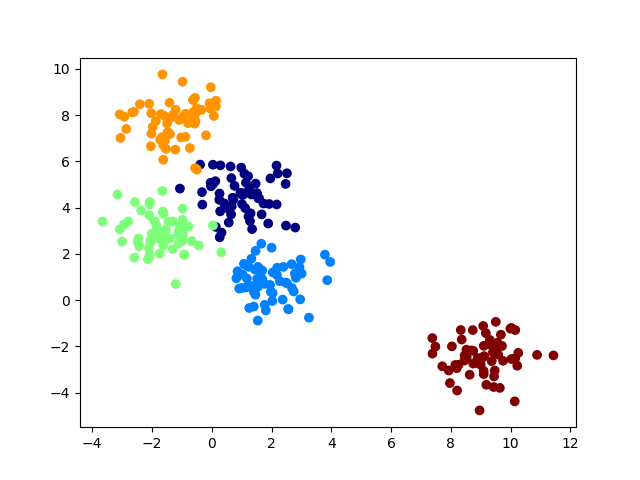
\includegraphics[scale=0.5]{images/short_simulation_generate_data.png}
    \caption{Data généré de manière synthétique}\label{fig:short_simulation_data}
\end{figure}

On viendra dans la suite chercher à trouver 4 clusters dans ces données.

\subsubsection{K-means}

L'algorithme K-means est un algorithme de clustering qui cherche à partitionner les données en K clusters.
L'algorithme fonctionne de la manière suivante :
\begin{enumerate}
    \item Choisir K points aléatoires dans les données, qui serviront de centres de clusters.
    \item Assigner chaque point de données au centre de cluster le plus proche.
    \item Mettre à jour les centres de clusters en prenant la moyenne des points assignés à chaque cluster.
    \item Répéter les étapes 2 et 3 jusqu'à ce que les centres de clusters ne changent plus.
\end{enumerate}


On obtient les résultats suivants :
\begin{figure}[h]
    \centering
    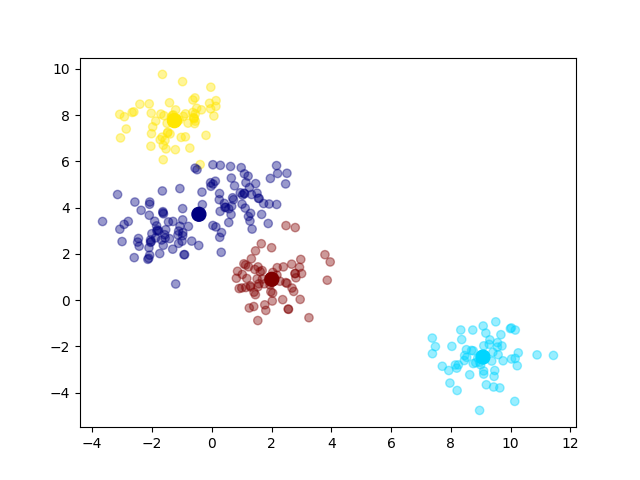
\includegraphics[scale=0.5]{images/short_simulation_kmeans.png}
    \caption{Résultat de l'algorithme K-means}\label{fig:short_simulation_kmeans}
\end{figure}

On remarque la fusion des deux clusters les plus proches ce qui est cohérent 
étant données que l'on cherche 4 clusters dans un ensemble de données regroupés en 5 clusters.
On verra que cette remarque s'appliquera à tous les algorithmes.


\subsubsection{K-medoids}

L'algorithme K-medoids est une variante de l'algorithme K-means. 
La différence principale est que K-medoids utilise des points de données comme centres de clusters, alors que K-means utilise des moyennes.
Cela rend K-medoids plus robuste aux valeurs aberrantes que K-means.
L'algorithme fonctionne de la manière suivante :
\begin{enumerate}
    \item Choisir K points aléatoires dans les données, qui serviront de centres de clusters.
    \item Assigner chaque point de données au centre de cluster le plus proche.
    \item Mettre à jour les centres de clusters en prenant le point de données qui minimise la somme des distances aux autres points assignés à chaque cluster.
    \item Répéter les étapes 2 et 3 jusqu'à ce que les centres de clusters ne changent plus.
\end{enumerate}

On a aussi appliquer cet algorithme sur le jeu de données précédent.
\begin{figure}[h!]
    \centering
    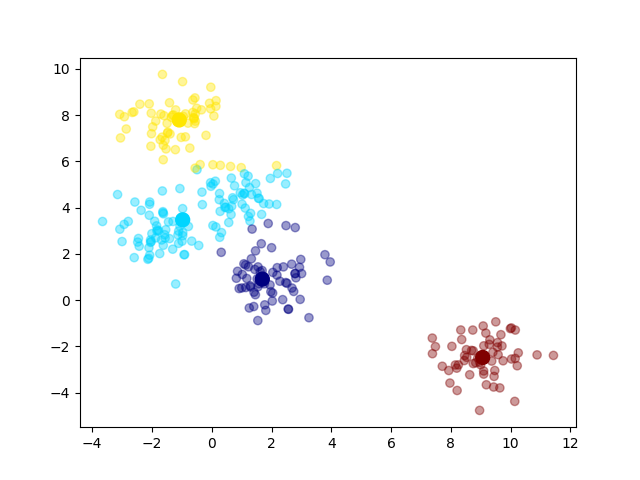
\includegraphics[scale=0.5]{images/short_simulation_kmedoids.png}
    \caption{Résultat de l'algorithme K-medoids}\label{fig:short_simulation_kmedoids}
\end{figure}

\subsubsection{Modèle à Mélange de Gaussiennes}

Un modèle de mélange gaussien (GMM) est un modèle probabiliste qui cherche à modéliser les données comme un mélange de distributions gaussiennes.
L'algorithme fonctionne de la manière suivante :
\begin{enumerate}
    \item Choisir K points aléatoires dans les données, qui serviront de centres de clusters.
    \item Assigner chaque point de données à une distribution gaussienne en utilisant la loi de Bayes.
    \item Mettre à jour les centres de clusters et les paramètres des distributions gaussiennes en maximisant la vraisemblance des données.
    \item Répéter les étapes 2 et 3 jusqu'à ce que les centres de clusters ne changent plus.
\end{enumerate}

Résultat de l'algorithme sur le jeu de données précédent.
\begin{figure}[h!]
    \centering
    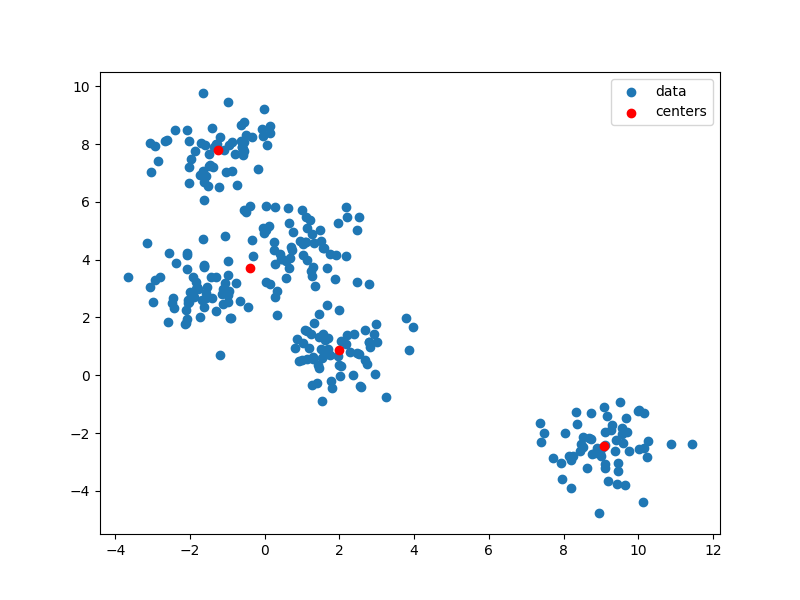
\includegraphics[scale=0.3]{images/short_simulation_gmm.png}
    \caption{Résultat de l'algorithme Modèle à Mélange de Gaussiennes}\label{fig:short_simulation_gmm}
\end{figure}

\subsubsection{DBSCAN}

DBSCAN est un algorithme de clustering qui est basé sur la densité des points. 
L'algorithme fonctionne de la manière suivante :
\begin{enumerate}
    \item Choisir un point de données aléatoire.
    \item Trouver tous les points de données qui sont à une distance inférieure à un seuil $\epsilon$ du point de données.
    \item Si le nombre de points de données trouvés est supérieur à un seuil $minPts$, alors on crée un cluster avec ces points de données et on recommence à l'étape 1 avec un autre point de données.
    \item Si le nombre de points de données trouvés est inférieur à $minPts$, alors on marque le point de données comme un point de bruit et on recommence à l'étape 1 avec un autre point de données.
\end{enumerate}

On a appliqué cet algorithme sur le jeu de données précédent avec une valeur de $\epsilon$ de 0.2 et une valeur de $minPts$ de 5.
Résultat de l'algorithme sur le jeu de données précédent.
\begin{figure}[h!]
    \centering
    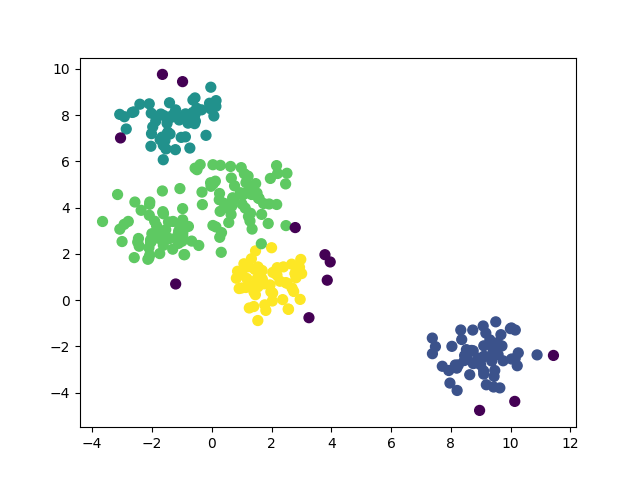
\includegraphics[scale=0.5]{images/short_simulation_dbscan.png}
    \caption{Résultat de l'algorithme DBSCAN}\label{fig:short_simulation_dbscan}
\end{figure}

On remarque ici que certains points ne sont pas assignés à un cluster, ce sont les points de bruit.

\section{Application sur la base de données MNIST}
\subsection{K-means}
Afin de baisser le temps de calcul, on ne va étudier que les 10 000 premières images de la base de données MNIST.
On aura donc 10 clusters contenant chacun : 
\begin{itemize}
    \item label 0 : 1001 images
    \item label 1 : 1127 images
    \item label 2 : 991 images
    \item label 3 : 1032 images
    \item label 4 : 980 images
    \item label 5 : 863 images
    \item label 6 : 1014 images
    \item label 7 : 1070 images
    \item label 8 : 944 images
    \item label 9 : 978 images
\end{itemize}

On clusterise les images en utilisant les pixels comme features et on recherche 10 clusters.
\begin{figure}[h!]
    \centering
    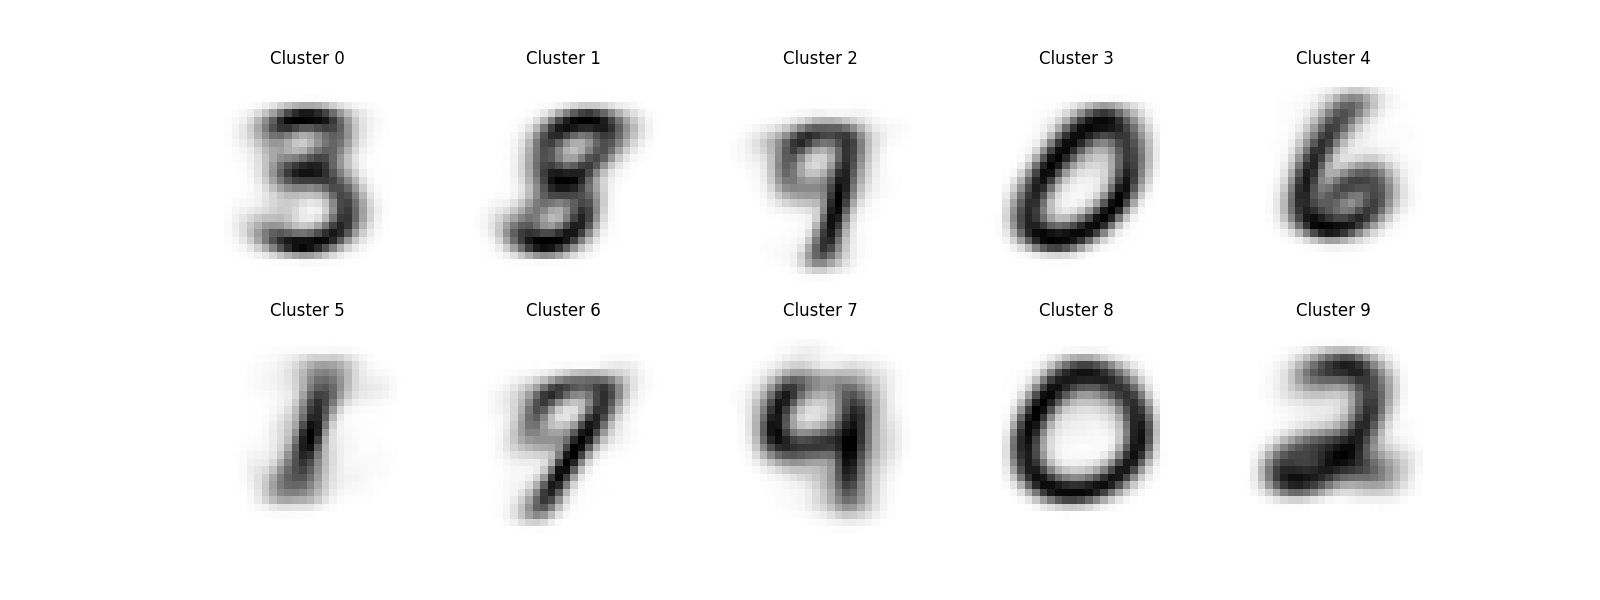
\includegraphics[scale=0.2]{images/mnist_kmeans_ten_clusters.png}
    \caption{Résultat de l'algorithme K-means sur la base de données MNIST}\label{fig:mnist_kmeans}
\end{figure}
\subsection{K-medoids}


\end{document}
